% THIS IS SIGPROC-SP.TEX - VERSION 3.0
% WORKS WITH V3.1SP OF ACM_PROC_ARTICLE-SP.CLS
% JUNE 2007
%
% It is an example file showing how to use the 'acm_proc_article-sp.cls' V3.1SP
% LaTeX2e document class file for Conference Proceedings submissions.
% ----------------------------------------------------------------------------------------------------------------
% This .tex file (and associated .cls V3.1SP) *DOES NOT* produce:
%       1) The Permission Statement
%       2) The Conference (location) Info information
%       3) The Copyright Line with ACM data
%       4) Page numbering
% ---------------------------------------------------------------------------------------------------------------
% It is an example which *does* use the .bib file (from which the .bbl file
% is produced).
% REMEMBER HOWEVER: After having produced the .bbl file,
% and prior to final submission,
% you need to 'insert'  your .bbl file into your source .tex file so as to provide
% ONE 'self-contained' source file.
%
% Questions regarding SIGS should be sent to
% Adrienne Griscti ---> griscti@acm.org
%
% Questions/suggestions regarding the guidelines, .tex and .cls files, etc. to
% Gerald Murray ---> murray@acm.org
%
% For tracking purposes - this is V3.0SP - JUNE 2007

% \documentclass{acm_proc_article-sp}
\documentclass{sig-alternate}

\graphicspath{{figures/}}

\begin{document}

\title{Software Trajectory Analysis:\\An empirically based method for automated software process discovery}

%\numberofauthors{8} %  in this sample file, there are a *total*
% of EIGHT authors. SIX appear on the 'first-page' (for formatting
% reasons) and the remaining two appear in the \additionalauthors section.
%
\numberofauthors{1}
\author{
% You can go ahead and credit any number of authors here,
% e.g. one 'row of three' or two rows (consisting of one row of three
% and a second row of one, two or three).
%
% The command \alignauthor (no curly braces needed) should
% precede each author name, affiliation/snail-mail address and
% e-mail address. Additionally, tag each line of
% affiliation/address with \affaddr, and tag the
% e-mail address with \email.
%
% 1st. author
\alignauthor Pavel Senin \\
%\titlenote{Corresponding author. Email: senin@hawaii.edu}\\
	\affaddr{IRISA, campus de Beaulieu}\\
	\affaddr{35042 Rennes Cedex, France}\\
	\email{pavel.senin@inria.fr}\\
% 2nd. author
%\alignauthor Philip M. Johnson \titlenote{PhD Thesis adviser.}\\
%	\affaddr{CSDL, University of Hawaii at Manoa}\\
%	\affaddr{1680 East-West Rd, Honolulu, HI 96822}\\
%	\email{johnson@hawaii.edu}
}
% There's nothing stopping you putting the seventh, eighth, etc.
% author on the opening page (as the 'third row') but we ask,
% for aesthetic reasons that you place these 'additional authors'
% in the \additional authors block, viz.
%\additionalauthors{Additional authors: John Smith (The Th{\o}rv{\"a}ld Group,
%email: {\texttt{jsmith@affiliation.org}}) and Julius P.~Kumquat
%(The Kumquat Consortium, email: {\texttt{jpkumquat@consortium.net}}).}
%\date{30 July 1999}
% Just remember to make sure that the TOTAL number of authors
% is the number that will appear on the first page PLUS the
% number that will appear in the \additionalauthors section.
\maketitle
\begin{abstract}
A process defines a set of routines which allow to organize, manage and improve activities to reach a goal. With an expert intuition and apriori knowledge software processes were modeled for the long time resulting in Waterfall, Spiral and other development models. Later, with a wide use of SCM systems and public availability of primitive software process artifact trails, formal methods such as Petri Nets, State Machines and others were applied for recurrent processes discovery and control. Recent advances and increase in use of continuous integration and in-process software measurement and analysis systems rich types of software process artifacts becoming available. In this work I propose to investigate an automated technique for the discovery and characterization of recurrent behaviors in software development - ``programming habits'' either on an individual or a team level.
\end{abstract}

% A category with the (minimum) three required fields
%\category{H.4}{Information Systems Applications}{Miscellaneous}
%A category including the fourth, optional field follows...
%\category{D.2.8}{Software Engineering}{Metrics}[complexity measures, performance measures]

%\terms{Software process}

%\keywords{ACM proceedings, \LaTeX, text tagging} % NOT required for Proceedings

\section{Introduction and Motivation}
A \textit{software process} is a set of activities performed in order to design, develop and maintain software systems. Examples of such activities include design methods; requirements collection and creation of UML diagrams; testing and performance analysis. The intent behind a software process is to structure and coordinate human activities to achieve the goal - deliver a software system successfully; while the objective of software process research is to design a process consisting of a set of recurrent behaviors which allows to reproduce such a success consistently and improve the process performance.

Much work has been done in software process research resulting in a number of industrial standards for process models (CMM, ISO, PSP etc. \cite{citeulike:5043104}) which are widely accepted by many government and industrial institutions. Nevertheless, software development remains error-prone and more than a half of all software development projects ending up failing or being very poorly executed. Some of them are abandoned due to running over budget, some are delivered with such low quality or so late that they are useless, and some, when delivered, are never used because they do not fulfill requirements \cite{citeulike:7351135}. The cost of this lost effort is enormous and may in part be due to our incomplete understanding of software process.

There is a long history of software process improvement through proposing specific patterns of software development. For example, the Waterfall Model process proposes a sequential pattern in which developers first create a Requirements document, then create a Design, then create an Implementation, and finally develop a Tests. On the contrary, the Test Driven Development process proposes an iterative pattern in which the developer must first write a test case, then write the code to implement that test case, then refactor the system for maximum clarity and minimal code duplication. Probably the main problem with this traditional top-down approach to process development is that it requires the developer or manager to notice a recurrent pattern of behavior in the first place \cite{citeulike:5043104}. 

As an alternative to that, in my research, I am applying knowledge discovery and data mining techniques to the domain of software engineering in order to evaluate their ability to automatically notice interesting recurrent patterns of behavior from collected software process artifacts. While I am not proposing to be able to infer a complete and correct software process model, my system will provide its users with a formal description of recurrent behaviors in their software development. As a simple example, consider a development team in which committing code to a repository triggers a build of the system. Sometimes the build passes, and sometimes the build fails. To improve the productivity of the team, it would be useful to be aware of any recurrent behaviors of the developers. My system might generate one recurrent pattern consisting of a) implementing code b) running unit tests, c) committing code and d) a passed build: $i \rightarrow u \rightarrow c \rightarrow s $, and another recurrent pattern consisting of a) implementing code, b) committing code, and c) a failed build: $i \rightarrow c \rightarrow f $. The automated generation of these recurrent patterns can provide actionable knowledge to developers; in this case, the insight that running test cases prior to committing code reduces the frequency of build failures.

\section{Relevant prior work}
Although process mining in the business domain is a well-established field with much software developed up to date (ERP, WFM and other systems), ``Business Process Intelligence'' tools usually do not perform process discovery and typically offer relatively simple analyzes that depend upon a correct a-priori process model \cite{citeulike:3718014} \cite{citeulike:5044991} \cite{citeulike:2678511}. This fact restricts direct application of business domain process mining techniques to software engineering, where processes are usually performed concurrently by many agents, are more complex and typically have a higher level of noise. Taking this fact in account, I will review only the approaches to the process mining for which applicability to software process was expressed. 

Perhaps, the research most relevant to my own was done by Cook \& Wolf in \cite{citeulike:328044}. The authors developed a \textit{``process discovery''} techniques intended to discover process models from event streams. The authors did not attempt to generate a complete model, but rather to generate sub-models that express the most frequent patterns in the event stream. They designed a framework which collects process data from history logs, and generates a set of recurring patterns of behavior characterizing observed process. In this work they extended two methods of \textit{grammar inference} from previous work: purely statistical (neural network based \textit{RNet}) and purely algorithmic (\textit{KTail}) as well as developing their own Markovian method (\textit{Markov}). 

\begin{figure}[tbp]
   \centering
   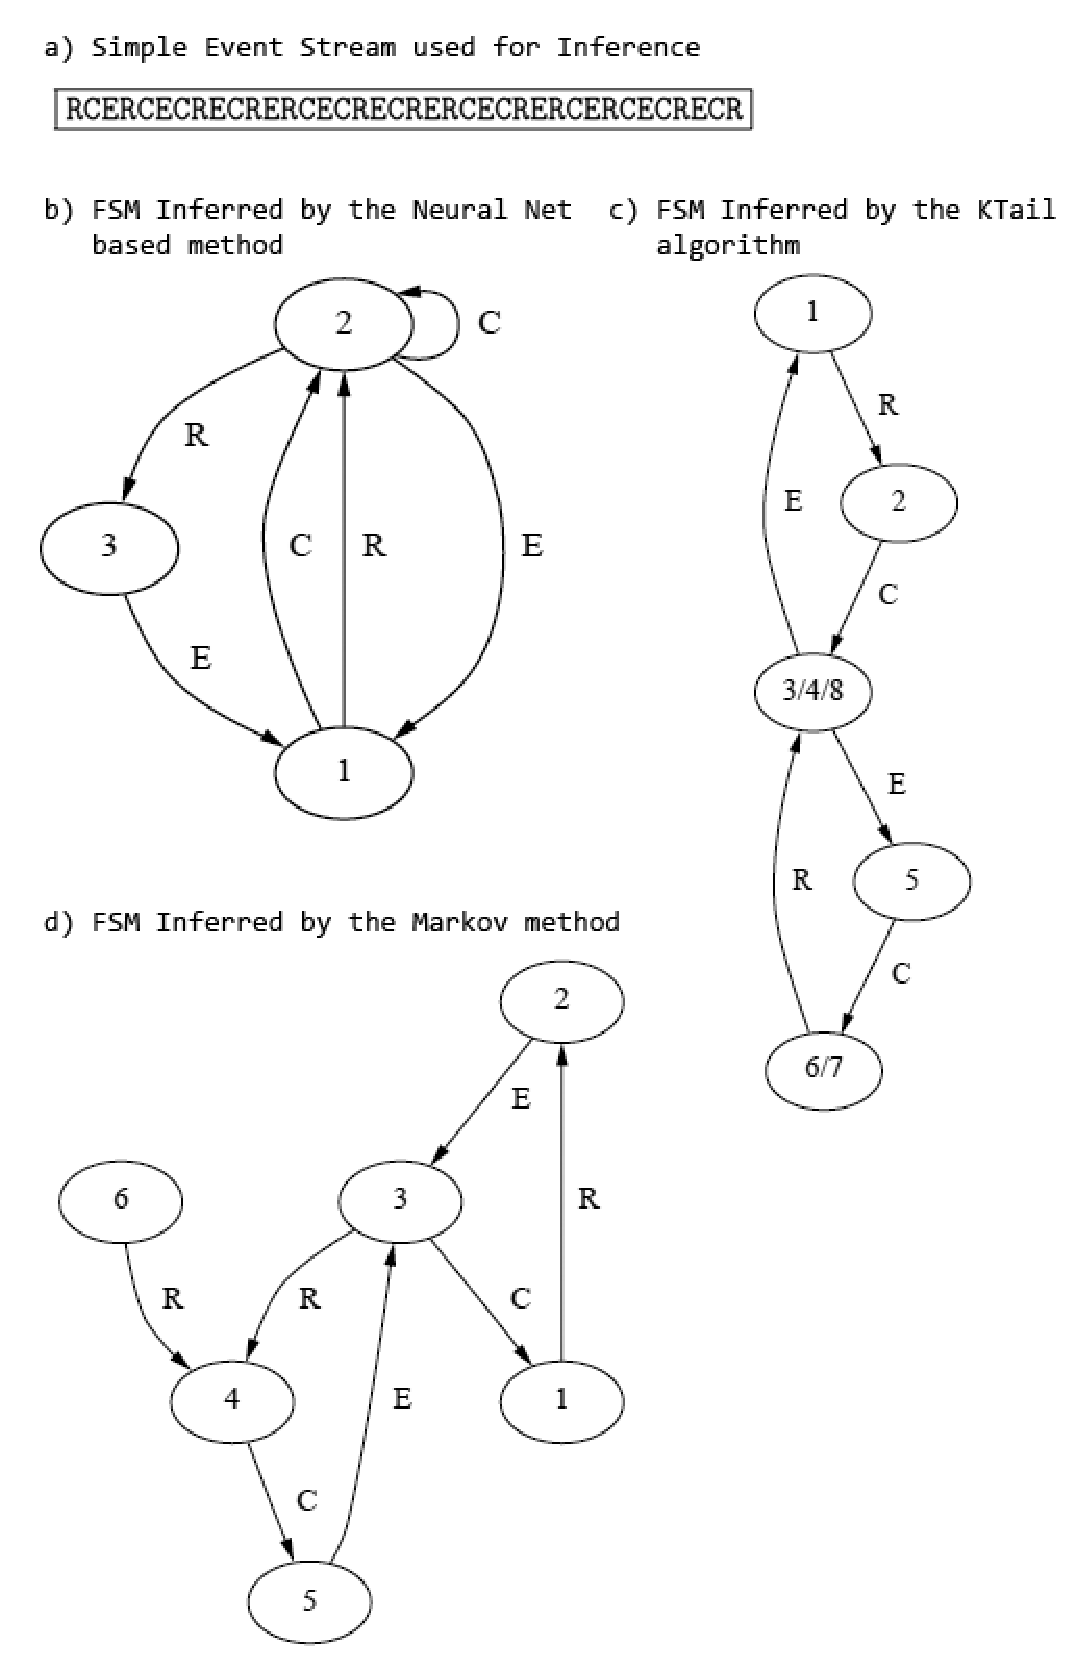
\includegraphics[height=45mm]{inference.eps}
   \caption{Process discovery through the grammar inference: panel a) a sample event stream (simple process involving three types of events: Edit, Review, and Checkin); and FNA results obtained by applying three methods of process discovery from Cook \& Wolf \cite{citeulike:328044}.}
   \label{fig:inference}
\end{figure}

The first method extended by the authors, the neural-network based grammar inference, RNet algorithm, defines a recurrent neural network architecture which is trained by the sequences of events. After training, this neural net is able to characterize a current system state by looking on past behavior. The authors extract the FSM from the trained neural network by presenting different strings to it and extracting the hidden neurons activity through observations. Due to the nature of Neural Net, closely related activation patterns are clustered into the same state; therefore, by noting the current pattern, the input token, and the next activation pattern, transitions are recorded and compiled into the inferred FSM.

The second method investigated, is a purely algorithmic KTail method, which was taken from the work of Biermann \& Feldman \cite{citeulike:5120603}. The idea is that a current state is defined by what future behaviors can occur from it. The \textit{future} is defined as the set of next $k$ tokens. By looking at a window of successor events, the KTail algorithm can build the equivalence classes that compose the process model. The authors extensively modified the original KTail algorithm improving the folding in the mined model making it more robust to noise.

The Markov based method developed by the authors is based on both algorithmic and statistical approaches. It takes to account past and future system behavior in order to guess the current system state. Assuming that a finite number of states can define the process, and that the probability of the next state is based only on the current state (Markov property), the authors built a $n^{th}$-order Markov model using the first and second order probabilities. Once built, the transition probability table corresponding to the Markov model is converted into FSM which is in turn reduced based on the user-specified cut-off threshold for probabilities.

The authors implemented all three of these algorithms in a software tool called \textsc{DaGama} as a plugin for larger software system called Balboa \cite{citeulike:5120757}. By performing benchmarking, Cook \& Wolf found that the Markov algorithm was superior to the two others. RNet was found to be the worst of the three algorithms. The software tool was applied to a real-world process data and demonstrated an abstraction of the actual process executions and ability to capture important properties of the process behavior. The major backdraw of the approach, as stated by the authors, lies in the inability of the FSMs to model concurrency of processes which limits its applicability to the software development process. Later, Cook et al. in \cite{citeulike:5128143} addressed this limitation by using Petri-nets and Moore-type FSM.

\begin{figure}[tbp]
   \centering
   \includegraphics[height=36mm]{petri.eps}
   \caption{Illustration of the ``Generation and Synthesis Approach'' from \cite{citeulike:5043673}: a) Transition System with regions shown; b),c) Petri Nets synthesized from the Transition System.}
   \label{fig:petri}
\end{figure}

Another set of findings relevant to my research approach was developed by Rubin et al. \cite{citeulike:1885717} and van der Aalst et al. \cite{citeulike:3718014} and is called \textit{incremental workflow mining}. The authors not only designed sophisticated algorithms but built a software system using a business process mining framework called ProM by van Dongen et al. \cite{citeulike:5043673} which synthesizes a Petri Net corresponding to the observed process. The system was tested on SCM logs and while the process artifacts retrieved from the SCM system are rather high-level, the approach discussed is very promising for the modeling of software processes from the low-level product and process data.

The algorithm input is an event chain constructed through the ``abstraction on the log level'', which aggregates basic events into single high-level entities, is treated with the \textit{Generate} part of the \textit{``Generate and Synthesis''} \cite{citeulike:3718014} algorithm in order to generate a \textit{Transition System} which represents an ordered series of events. This algorithm looks at the history (prefix) and the future (suffix) sequences of events related to the current one in order to discover transitions.  When applied to the abstracted log information, the algorithm generates a rather large Transition System graph where edges connect to abstracted events. This transition system is then successively simplified by using various reduction strategies. At the last step of the incremental workflow mining approach, Transition Systems are used to \textit{Synthesize} labeled Petri nets (where different transition can refer to the same event) with the help of \textit{``regions theory''} \cite{citeulike:5128170}. As with the Transition System generation, the authors investigate many different strategies of Petri nets synthesis, showing significant variability in the results achieved. (see Figure \ref{fig:petri}). The significant contribution of this research is in the generality of the method. It was shown that by tuning the ``Generate'' and ``Synthesize'' phases it is possible to tailor the algorithm to a wide variety of processes. In particular, as mentioned before, Rubin et al. successfully applied this framework to the SCM logs and audit trails analysis.

In addition to discussed work latest trends in software process research emphasize mining of software process artifacts and behaviors \cite{citeulike:5043664} \cite{citeulike:5112229}. 

It worth noting that while reviewed work outlined approaches for concurrent processes modeling, to the best knowledge of the author of this article the application to the software process artifacts did not yield sensible results. This may be partially due to the high level of noise or to the lack of means of fine-grained software process artifacts collection. In my approach I am planning to address both issues by leveraging the ability of the Hackystat system \cite{citeulike:4041809} to collect such a fine grained data and by the ability to perform symbolic reduction and indexing of temporal data.

\section{Research objectives}
As shown by previous research, it is possible to infer and successively formalize sequential software process by observing its artifacts, and in particular, recurrent behavioral patterns. The problem of finding such patterns is the cornerstone of my research. Solving this will extend previous research with new knowledge that will support improvements in our understanding of software process.

The main research objectives of my work is a design, development and evaluation of a previously unexplored approach to discovering of recurrent behaviors in software process through the temporal data mining of low-level process and product artifacts. 

To reach this ultimate goal I am planning to perform a number of steps starting from an exploratory study of applicability of proposed pattern-mining techniques to the various levels of complexity of software process artifacts; developing an expert software package afterward, and performing an empirical study to evaluate the approach at the end.

\section{Research approach}
My approach to this problem rests on the application of data-mining techniques to symbolic time-point and time-interval series constructed directly from the real-valued telemetry streams provided by Hackystat or by a similar system.

To investigate the requirements for a software tool that aids in the discovery of recurrent behavioral patterns in software process, I am designing and developing the ``Software Trajectory'' framework. A high-level overview of the framework is shown in Figure \ref{fig:system_overview} and resembles the flow of the ``Knowledge Discovery in Database'' process discussed by Han et al. in \cite{citeulike:709476}. As shown, the data collected by Hackystat is transformed into a symbolic format and then indexed for further use in data-mining. The tools, designed for data-mining, have a specific restrictions placed on the search space by domain and context knowledge in an attempt to limit the amount of reported patterns to useful ones. I am planning to design a GUI in a way that will allow easy access and modification of these restrictions. 

While I intend to use Hackystat as a primary data collection system in my future experimental setup, for the current exploratory study I am looking on other ways of data collection, extraction and abstraction. The ability to abstract into symbolic representation various software artifact streams such as SCM logs and audit trails is crucial for the exploratory study phase by enabling me to experiment with much broader spectrum of existing software process data collections refining developed data-mining techniques.

\begin{figure}[tbp]
   \centering
   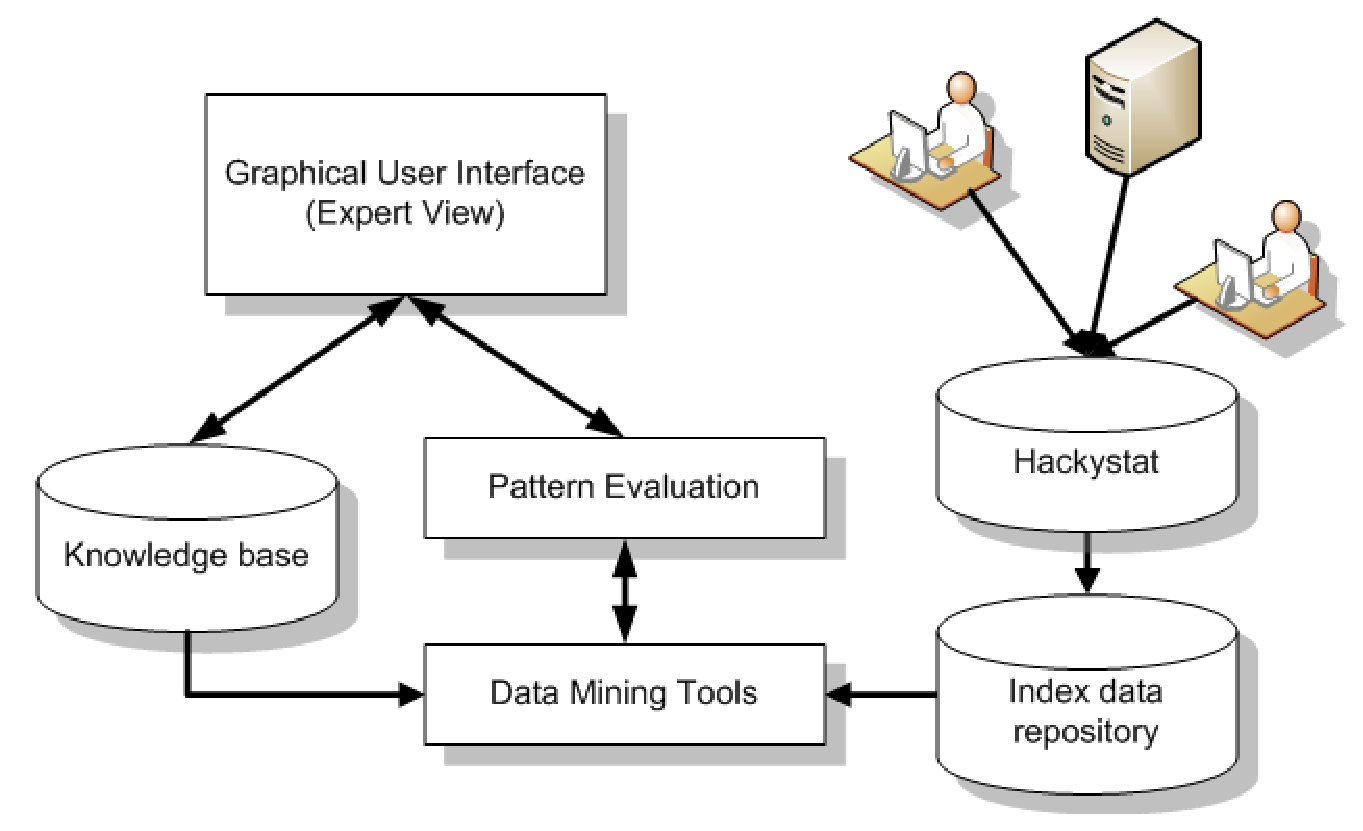
\includegraphics[height=50mm]{system_overview.eps}
   \caption{The high-level system overview. Software engineering process and product data are collected and aggregated by Hackystat and then used to generate temporal symbolic indexes. Data mining tools constrained by software engineering domain knowledge are then used for unsupervised patterns discovery. The GUI provides an interface to the discovered patterns and aids in investigation of a discovered phenomena.}
   \label{fig:system_overview}
\end{figure}
 
\section{Data and analysis methods}
As mentioned before, this research based on the mining of recurrent behavioral patterns from a symbolic representation of software processes as a temporal sequences of events performed by individual developers or automated tools with or without concurrency. 

Various types of data are suitable for software process analyzes. For example, simplest data extracted from SCM logs allow to track software change and perform a basic software process reconstruction - however a very little information can be recalled about development activities and behaviors from such data and models. When development audit trails added to analyzes - enriched data allow to shed more light on the performed process, while adding considerable amount of noise to the models. By using logs of an automated build system it is possible to collect a broader spectrum of artifacts and software metrics such as cyclomatic complexity or coverage, moreover centralized build system creates a set of singular points which are tying together in time processes performed concurrently by developers. Finally, collecting temporal data about atomic development events by the means of Hackystat and similar systems - such as background compilation and test results, buffer transfers along with quantification of the actual effort enables rich characterization of the dynamic behavior of a software process in great detail. However, as shown by previous experience - the amount of noise will be unbearable high for conventional methods of process inference.

Having this limitation in mind, approach I am taking in my research differs from previous attempts by it's relative simplicity and inspired by recent advances in two research fields: in temporal patterns mining from time-series and in motif finding in biological sequence analysis. 

Current state of the art approach in temporal data mining called Symbolic Aggregate approXimation and was proposed by Lin et al. in \cite{citeulike:2821475}. This method extends the PAA-based approach, inheriting algorithmic simplicity and low computational complexity, while providing satisfiable sensitivity and selectivity in range-query processing. Moreover, as mentioned by the authors, the use of a symbolic representation opens the door to the existing wealth of data-structures and string-manipulation algorithms in computer science such as hashing, regular expression pattern matching, suffix trees etc. As showed by the authors, SAX outperforms all previously known methods - DFT, DWT, DTW and similar - by using SAX it is possible to index and find recurrent and ``surprise'' patterns in vast amounts of data in almost linear time and space \cite{citeulike:1630245} \cite{citeulike:3025877} \cite{citeulike:3000416}. Looking at the SAX-performed data reduction one might notice that due to the PAA step of the algorithm high level of noise is reduced dramatically - leaving only major time-series trends for ``symbolization''. In my opinion, this protocol can be adopted for the complexity reduction of the software process artifacts streams. For example, if symbolic approximation of performed process would be $i \rightarrow i \rightarrow i \rightarrow u \rightarrow i \rightarrow i \rightarrow i \rightarrow u \rightarrow c \rightarrow s $ indicating long cycle of development with intermediate unit test at some point (position 4) it is possible to dismiss this unit test event and collapse in time all development events into the single one - $i \rightarrow u \rightarrow c \rightarrow s $ reducing the pattern complexity. Another idea borrowed from the SAX and Bioinformatics sequence alignment is in the distance function implementation - which will score sequences different by a single symbol (single substitution) as equal if the both symbols are approximately equal to each other in the context of actions. For example, one can say that running static code analysis tools such as CheckStyle, PMD or running Unit test is equal in the meaning - checking code quality and one common symbol would be assigned to all such events.

Multiple alignments of protein sequences are important in many biological applications, including phylogenetic tree estimation, secondary structure prediction and critical residue identification. Recent advances in MSA algorithms \cite{citeulike:692} include a new method for design and evaluation of objective functions for improving alignments by its profiling. Within the multiple alignment of biological sequences algorithm is introducing gaps and substitution within possibly similar sequences to find best score for alignment. If one will introduce gaps into the development motifs - for example ignoring presence or lack of code analysis events within a development cycle - it will immediately boost the evidence for both types of patterns - making them much more noticeable while preserving overall correctness.

\section{Preliminary results}
During my work on the pilot version of Software Trajectory framework, I began a set of small exploratory experiments in order to aid in the architectural design and algorithms implementation. In addition, these experiments helped me to outline the boundaries of applicability of my approach to certain problems in software engineering. I call these experiments \textit{Pilot study}.

\begin{figure}[tbp]
   \centering
   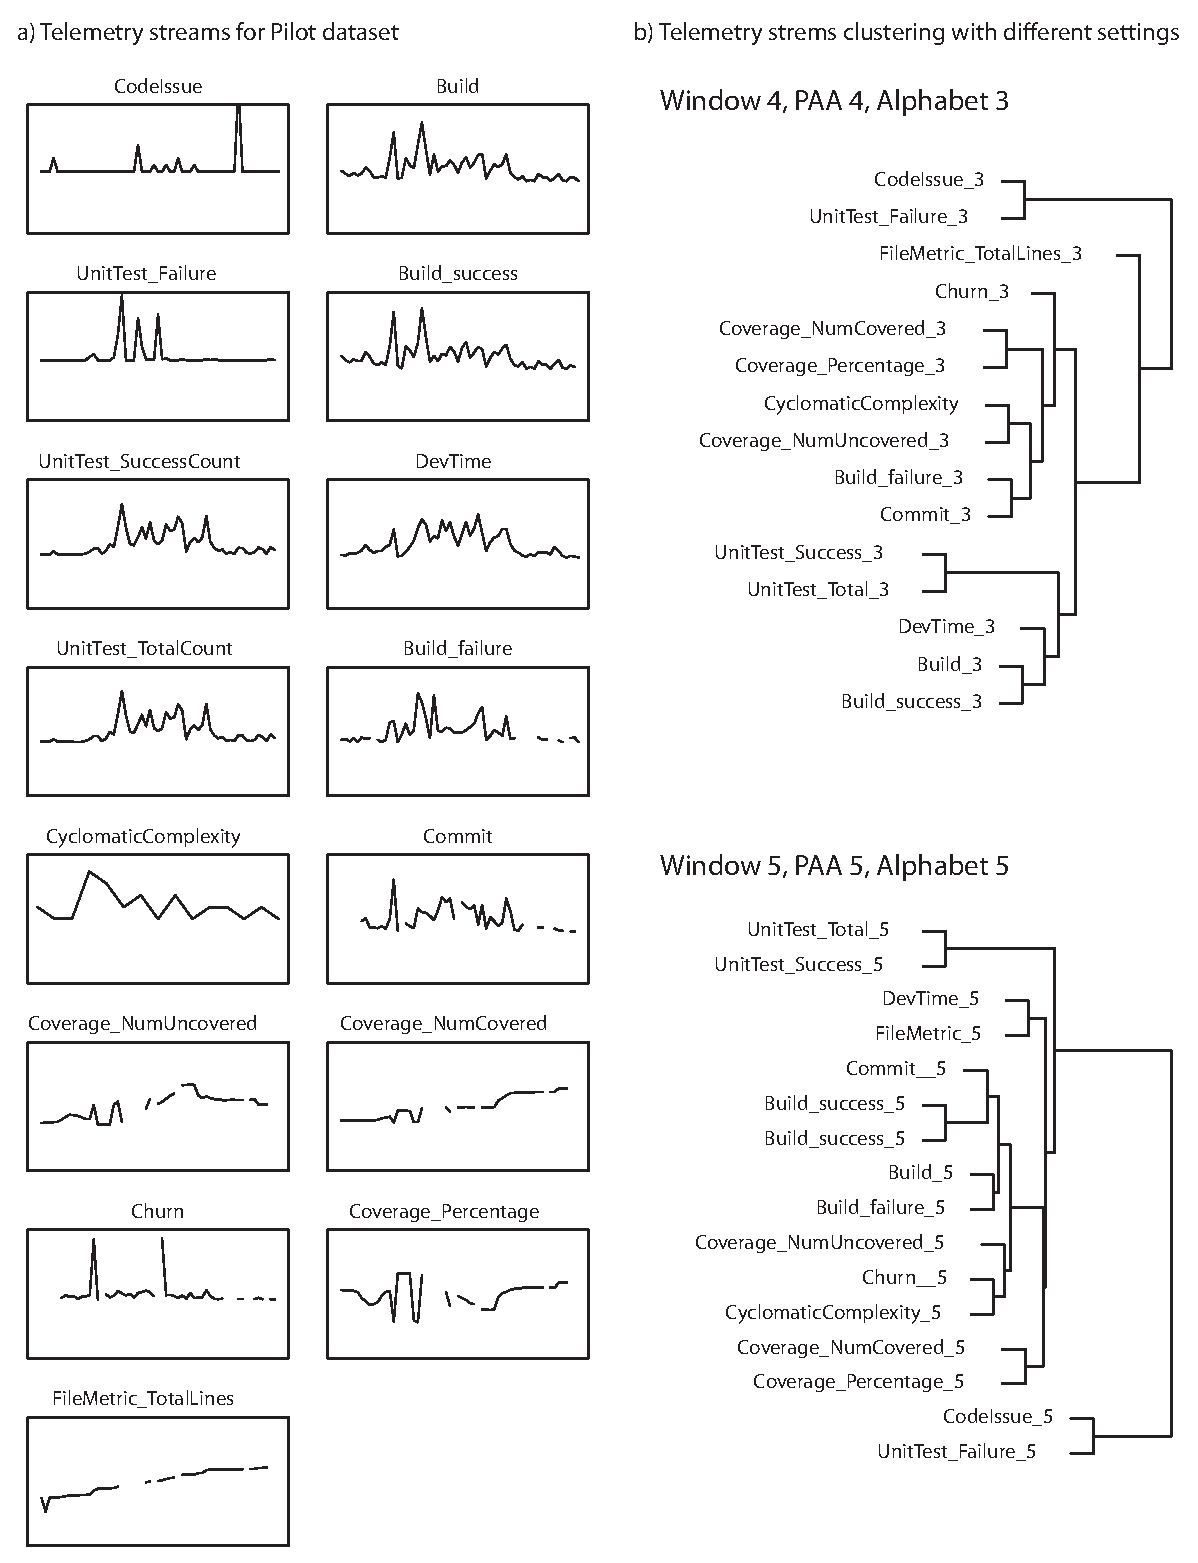
\includegraphics[height=100mm]{cluster_streams.eps}
   \caption{Clustering of telemetry streams for classroom pilot dataset using symbolic approximation and vectors of motif frequencies. While it seems to be meaningful to find correlation between \textit{UnitTest\_Failure} and \textit{CodeIssue} streams unit test, this grouping happened due to the similarity of behavior pattern - short, high amplitude bursts; but note, there is no correlation of features in time .}
   \label{fig:cluster_streams}
\end{figure}

One of the experiments was performed to evaluate the ability of PAA and SAX approximations and indexing to capture a temporal specificity of development time telemetry streams through the discovery of recurrent temporal patterns. Knowing about the frequently misleading results of a time-series clustering \cite{citeulike:227029}, I did not expect to capture many interesting facts, nevertheless the results were encouraging. The streams under analysis were composed by quantifying development events within a day: for example for the BuildSuccess stream a single value 5 means that five builds succeeded within that day. The data used in this study was collected from eight students and represents Hackystat metrics collected during sixty days of a classroom project. The two clustering experiments were conducted using the distance between vectors of motif frequencies (note that temporal ordering not accounted in these analysis) extracted by indexing of telemetry streams. The motif time period was one week.

At first, by clustering of development-time telemetry streams collected from individual developers I was able to group developers with similar behavioral patterns within clusters, which indicates the feasibility of the classification by effort approach. Figure \ref{fig:cluster_developers} depicts results of this analysis.

Clustering of product-related telemetry streams however was not successful. I was able to group telemetry streams, but while these groups look intuitively meaningful - for example clustering together filemetrics and development time - the close examination of the stream features suggests that this grouping happened due to the similar temporal behavior on the short stretches rather then positive correlation. This result, while proving the correctness of approach, indicates it's limitation, pointing that instead of using just motif frequencies, some temporal ordering should be taken into account. Figure \ref{fig:cluster_streams} displays results of this analysis.

Another result was also achieved by the direct application of indexing of symbolic approximation of the data streams. For this experiment I was using data collected from my own concurrent development of Trajectory software package and JMotif library. Within a symbolic approximation paradigm the change of symbols can be interpreted as growth or drop in the underlying data stream: for example consecutive $ab$ symbols indicate that growth happened and $ba$ correspond to a drop. The idea was to find if there were any drop or growth coincidences within two streams. For this purpose I defined a sliding window consisting of three days and searched such coinciding within a window events. Events were found within a development time stream, churn, commit and others. Detailed analysis of coinciding growth events revealed that changes within JMotif data manipulation routines almost always followed by changes within Trajectory data analyzes routines which heavily relying on the JMotif API. While within my software project portfolio such a discovery is a quite obvious fact one can see the immediate application of such a method to large portfolio or software system - by performing such analyzes it will be possible to build a repertoire of frequent consecutive changes and also estimate an effort required for performing such changes extrapolating previous experience.

\begin{figure}[tbp]
   \centering
   \includegraphics[height=48mm]{dev_clustering.eps}
   \caption{Clustering of developers behavior using symbolic approximation and vectors of motif frequencies. This analysis captured similar development behavior among developers. Developers \#2 and \#7 were consistent (no bursts observed) in both, coding and measuring effort during whole time interval, while all others can be characterized with bursty, inconsistent effort.}
   \label{fig:cluster_developers}
\end{figure}

\section{Exploratory study directions}
Previous section describes two finished experiments which give an inside on the applicability of SAX approximation of Telemetry streams to recurrent behavior in software process reconstruction. While working on both experiments, I have designed a database schema which supports symbolic indexing of telemetry streams. By having such a storage I have an immediate access to the symbolic streams reflecting software process which allows me to perform time-range queries with use of Regular Expressions (in SQL language) and extract sequences of interest which for example include successful Unit-Tests, Commits, or CyclomaticComplexity above an arbitrary threshold. Such a database is somewhat similar to the CVSAnalY tool \cite{citeulike:6544724}. One of the direction I am working on right now is the concurrent use of the both databases under unifying API in order to evaluate a capacity of such approach in the recurrent behavior discovery for the MSR challenge \cite{citeulike:5043676}.

Mentioned before, recent advances in biological data mining in created a wealth of the algorithms and complete software tools. According to \cite{citeulike:964046} there are two categories of approaches for motif finding in biological sequences and in particular, the second approach which ``uses patterns with `mismatch representation' which define a signal to be a consensus pattern and allow up to a certain number of mismatches to occur in each instance of the pattern'' - looks very promising as an extension of exact motifs search explained before. By allowing mismatches the noise from non-frequent events will not decrease evidence value for the similar patterns allowing to identify key events of the observed process (as similar to the key amino-acids residues within protein sequences) I am planning to perform an experiment consisting of abstraction of software process artifacts into the symbolic representation mimicking protein encoding and apply multiple motif-finding packages after evaluating their ability to recall some frequent behaviors.

Concurrent software process occurs within a team working on a common goal. Within such a process developers interact at many levels, but in the context of this work the focus put on the role of SCM and build automation (such as continuous integration) in their ability to serve as a place which persists among all levels and creates means of interaction for all agents. I plan to perform analyzes on telemetry streams coming from individual agents using SCM and automation events as the time-points breaking such individual continuous streams onto short intervals representing fragment sets of concurrent process. I expect to find difference among such a fragment sets reflecting different phases of development as well as differences among sets from individual agents reflecting team-assigned roles.

\section{Future empirical study design}
It is proposed to conduct two case studies: \textit{Public data case study}, and \textit{Classroom case study} in order to empirically evaluate the capabilities and performance of Software Trajectory framework. These studies differ in the granularity of data used, and in the approaches for evaluation. 

My intent behind these empirical studies is to assess the ability of Software Trajectory framework to recognize well known recurrent behavioral patterns and software processes (for example Test Driven Development), as well as its ability to discover new ones. In addition, these studies will support a classification and extension of the current Hackystat sensor family in order to improve Software Trajectory's performance. It is quite possible that some of the currently collected sensor data will be excluded from the Software Trajectory datasets, while some new ones will be designed and developed in order to capture important features from the studied software development data streams. 

The proposed public data case study is based on the use of publicly available Software Configuration Management (SCM) audit trails of the big, ongoing software projects such as Eclipse, GNOME etc. Mining of SCM repositories is a well-developed area of research with much work published \cite{citeulike:5043676}. SCM repositories contain coarse software product artifacts which are usually mined with a purpose of discovering of various characteristics of software evolution and software process. I am using a mixed-method approach in this study. In the first phase of this study, I plan to perform SCM audit trail data mining following published work and using Software Trajectory as a tool in order to discover confirmed patterns in software process artifacts, and thus quantitatively evaluate Software Trajectory's performance when compared to existing tools. In the second phase, I will develop my own pre-processing and taxonomy mapping of software process artifacts into temporal symbolic series. By using this data and Software Trajectory framework, I plan to develop a new approach for SCM audit trail mining and possibly discover new evolutionary behaviors within software process. 

The classroom case study is based on a more comprehensive data set. This data will be collected by Hackystat from Continuous Integration and from individual developers and will contain fine-grained information about performed software process which may or may not reflect a development practice restriction placed by the lecturer. The approach I am taking in this study is very similar to the public data case study. I will develop my own taxonomy for mapping of software process artifacts into symbolic temporal data and will apply Software Trajectory analyzes to this data in order to discover recurrent behaviors. In turn, these discovered knowledge will be evaluated through interviewing for usefulness and meaningfulness. 

\section{Conclusions}
This paper presented a proposed approach to discovering novel recurrent behaviors in software process. Current study, while being in the exploratory phase reviled some insights into the applicability of proposed methods as well as a feasibility of aims. The wealth of developed techniques for temporal symbolic data mining, recent development of SAX approximation and advances in Bioinformatics allow me to overcome many computational limitations in existing approaches for mining of software process artifacts. The current implementation of Hackystat provides the ability to capture fine-grain software product and process metrics providing a richness of data, which, potentially, might reveal new insights. Summarizing experience collected within exploratory study with obtained concrete results I can only see that the properties of this approach and its current implementation in the Software Trajectory framework appear to be very promising. 

%\end{document}  % This is where a 'short' article might terminate

%ACKNOWLEDGMENTS are optional
%\section{Acknowledgments}
%This section is optional; it is a location for you
%to acknowledge grants, funding, editing assistance and
%what have you.  In the present case, for example, the
%authors would like to thank Gerald Murray of ACM for
%his help in codifying this \textit{Author's Guide}
%and the \textbf{.cls} and \textbf{.tex} files that it describes.

%
% The following two commands are all you need in the
% initial runs of your .tex file to
% produce the bibliography for the citations in your paper.
\bibliographystyle{abbrv}
\bibliography{seninp}  % sigproc.bib is the name of the Bibliography in this case
% You must have a proper ".bib" file
%  and remember to run:
% latex bibtex latex latex
% to resolve all references
%
% ACM needs 'a single self-contained file'!
%
%APPENDICES are optional
%\balancecolumns
%\appendix
%Appendix A
%\section{Headings in Appendices}
%The rules about hierarchical headings discussed above for
%the body of the article are different in the appendices.
%In the \textbf{appendix} environment, the command
%\textbf{section} is used to
%indicate the start of each Appendix, with alphabetic order
%designation (i.e. the first is A, the second B, etc.) and
%a title (if you include one).  So, if you need
%hierarchical structure
%\textit{within} an Appendix, start with \textbf{subsection} as the
%highest level. Here is an outline of the body of this
%document in Appendix-appropriate form:
%\subsection{Introduction}
%\subsection{The Body of the Paper}
%\subsubsection{Type Changes and  Special Characters}
%\subsubsection{Math Equations}
%\paragraph{Inline (In-text) Equations}
%\paragraph{Display Equations}
%\subsubsection{Citations}
%\subsubsection{Tables}
%\subsubsection{Figures}
%\subsubsection{Theorem-like Constructs}
%\subsubsection*{A Caveat for the \TeX\ Expert}
%\subsection{Conclusions}
%\subsection{Acknowledgments}
%\subsection{Additional Authors}
%This section is inserted by \LaTeX; you do not insert it.
%You just add the names and information in the
%\texttt{{\char'134}additionalauthors} command at the start
%of the document.
%\subsection{References}
%Generated by bibtex from your ~.bib file.  Run latex,
%then bibtex, then latex twice (to resolve references)
%to create the ~.bbl file.  Insert that ~.bbl file into
%the .tex source file and comment out
%the command \texttt{{\char'134}thebibliography}.
% This next section command marks the start of
% Appendix B, and does not continue the present hierarchy
%\section{More Help for the Hardy}
%The acm\_proc\_article-sp document class file itself is chock-full of succinct
%and helpful comments.  If you consider yourself a moderately
%experienced to expert user of \LaTeX, you may find reading
%it useful but please remember not to change it.
\balancecolumns
% That's all folks!
\end{document}
